        
        \documentclass[10pt, letterpaper]{article}
        \usepackage[utf8]{inputenc}
        \usepackage[margin=1in]{geometry}
        \usepackage{fancyhdr}
        \usepackage{titling}
        \usepackage{enumitem}
        \usepackage{mathtools}
        \usepackage{amssymb}
        \usepackage{xfrac}
        \usepackage{booktabs}
        \usepackage{graphicx}
        \usepackage{wrapfig, blindtext}
        \usepackage{hyperref}
        \usepackage{enumerate}
        
        
        
        
        % assignment info
        \title{Journal 2}
        \author{Sudhan Chitgopkar}
        \date{\today}
        
        % headers -- no need to change
        \pagestyle{fancy}
        \fancyhf{}
        \lhead{Council of Middle Earth}
        \chead{UGAMUNC XXVII}
        \rhead{\thedate}
        
        \begin{document}
        \noindent Dear Delegates, \\
        
        \noindent It’s my pleasure to welcome you all to the twenty-sixth annual UGA Model United Nations Conference, UGAMUNC XXVII! We hope that your experiences at this conference will teach you a little bit about both debating and the time period of the committee. With any luck, you’ll also have a lot of fun along the way. \\
        
        \noindent Before I get into the nitty gritty, I’d like to take a second to introduce myself. My name is Ian Allen (\texttt{\href{mailto:ian.allen00@uga.edu}{ian.allen00@uga.edu}}), and I’m a fourth-year International Affairs and Journalism major. This is my third year being involved with Model United Nations in any form, but I absolutely fell in love with the club and competitions as soon as I got a taste. Whenever I can find some spare time, I love reading, creative writing, cooking, rock climbing, and landscape photography. \\
        
        \noindent Your chair for the weekend will be Caroline Solomon (\texttt{\href{mailto: cks73791@uga.edu}{cks73791@uga.edu}}). She is a second year Environmental Economics \& Management major, Russian major, and Environmental Design minor. This is her first year of Model United Nations, and she really enjoys the team community and the fast-paced debate of the committees. In her free time, Caroline likes drawing, doing martial arts, and listening to sad podcasts. She can’t wait to chair for this committee and is looking forward to all the directions the committee will take! \\
        
        \noindent Your co-chair for the weekend will be Sarah Hartley (\texttt{\href{srh59784@uga.edu}{srh59784@uga.edu}}). She is a third-year pre-med student double majoring in Biology (area of emphasis in Neuroscience) and Comparative Literature with a minor in Spanish and this is her second year in Model UN. Model UN helped nurture a competitive and debative spirit in her as well as open the doors for connections and friends to be made. When she isn’t creating resolution plans or studying, you can find her reading, writing, or playing Animal Crossing. \\
        
        \noindent \textbf{Position papers will be due February 1, 2021.} Your position paper should explain what approach your character will take regarding personal actions, how you plan to interact with other delegates, and how you will respond to the main issues in the committee. Qualifying position papers for this committee will be one page and 1.5 spaced, 12 point Times New Roman font, one-inch margins, as well as a standard and consistent citation format of your choosing (i.e. MLA, Chicago, etc.). Email them to me as PDF files before the deadline! \\
        
        \noindent We know you’ll do an amazing job representing your characters in committee, and we also know you’ll have a great time at UGAMUNC as a whole! \\
        
        \noindent Finally, welcome to UGAMUNC XXVII! \\
        
        \noindent Sincerely, \\
        Ian Allen \\
        Crisis Director, Council of Middle-earth
        
        \newpage
        \tableofcontents
        \newpage
        
        \section{Rules \& Procedures}
        While other delegates at UGAMUNC may be placed in traditional General Assembly-style Model United Nations committees, the Council of Middle-earth committee at UGAMUNC is a crisis committee. While you should still familiarize yourself with the UGAMUNC Rules and Procedures to be familiar with parliamentary procedure, this committee will function uniquely both because of the topic and the fact that it will follow a crisis format. Please familiarize yourself with the following rules specific to this committee, and once again, if you have any questions, feel free to reach out to me at \texttt{\href{ian.allen00@uga.edu}{ian.allen00@uga.edu}}. I’m here to help! 
        \begin{itemize}
            \item {\textbf{This committee is directly based on the events and lore of the Lord of the Rings trilogy.} This includes The Hobbit, and The Silmarillion, prequels that set up and elaborate on the lore of the Tolkien universe. The committee itself is set after the events of the trilogy. I’m sure many of you have seen the six movies or read some of these books, and that will definitely help in creating crisis arcs and roleplaying inside this universe. If you haven’t seen or read any of these, I don’t expect you to spend the next couple of months cramming all this content in just for this committee. However, watching the original trilogy of movies is probably going to be the best bang for your buck in terms of prep time and payoff. Plus, they’re classics. Enjoy yourselves. Directly following the movies, perusing the LOTR wikia, which is cited often in this background guide, is a great source for more nitty-gritty details of lore.}
            
            \item {\textbf{While this is a fantasy committee, there are going to be limits to what you can do.} There are certain limitations placed on the universe and your powers. These are laid out in this guide and the basic rules of the Tolkien universe itself. Only one Wizard will be accessible to committee (Radagast, who is a committee member), all twenty Rings of Power are either destroyed or powerless, and the vast majority of characters in this universe lack significant magical powers. Obviously, we’re going to be open to creative ways of acquiring power and influence, but note that things are going to work a certain way. Note that crisis will put limitations on magical powers during the committee \textbf{at our discretion} to best ensure power balance among delegates. If it doesn’t belong in the setting and the mythology, we’ll steer you in another direction or simply not allow it.}
            
            \item {\textbf{Utilize crisis notes to accomplish your goals in committee and craft your crisis arc.} While the main method of negotiation in a typical General Assembly-style committee stems from work done during speaking time, in a crisis committee, much of the work you do will be on your own through crisis notes. These are letters that your character will write to crisis, a body outside of the committee room, to accomplish something without the committee’s knowledge. A good crisis note explains in detail what you want done and how to do it. These notes will be addressed to a fictional person connected to your character that you create. Crisis will answer these notes as if they were this person, responding as that person would under the circumstances and context you create. There are many fantastic resources that better explain crisis notes in detail, but a starting point can be found \texttt{\href{http://bestdelegate.com/the-three-crisis-notes-to-send-at-the-beginning-of-any-model-un-crisis-committee/}{here}}.}
            
            \item {\textbf{Because this is a crisis-style committee, write directives, not resolutions.} Although they are very similar, directives are the typical formal paper written in a crisis committee, not resolutions. Directives are less formal, normally titled, shorter, and generally more straightforward. They are intended to utilize the collective powers of the committee to address issues presented during the crisis.}
            
            \item {\textbf{Represent your understanding of your character.} Because these characters are largely fictional, it is up to you to take your character description and create a full personality to fit your role. Each character is unique, and subsequently has unique goals, relationships, and resources. That being said, be sure to represent your character’s beliefs and best interests rather than just your own. While you may not be prepared for the updates the crisis body will present, it is most important that you be familiar enough with your character to react as they would. }
            
            \item {\textbf{Attempt to be canonically accurate.} This may not be a historical committee, but it is still important that historicity is respected whenever possible. We’d like you to understand the location and time period in which the committee is set, and this might require doing prior research. This also means that some convenient technologies may not have been invented yet, and are therefore not available in committee. For example, posting a dope selfie with the hashtag \#dingdongthedarklordisdead via crisis would not be possible, but perhaps a pigeon message with an artistic rendering of the aforementioned image would be (although I’m unsure of the merits of including a hashtag, as pigeon messengers are unable to organize themselves categorically in this way).}
                \end{itemize}
    
            \newpage
            \section{Map}
            \begin{center}
             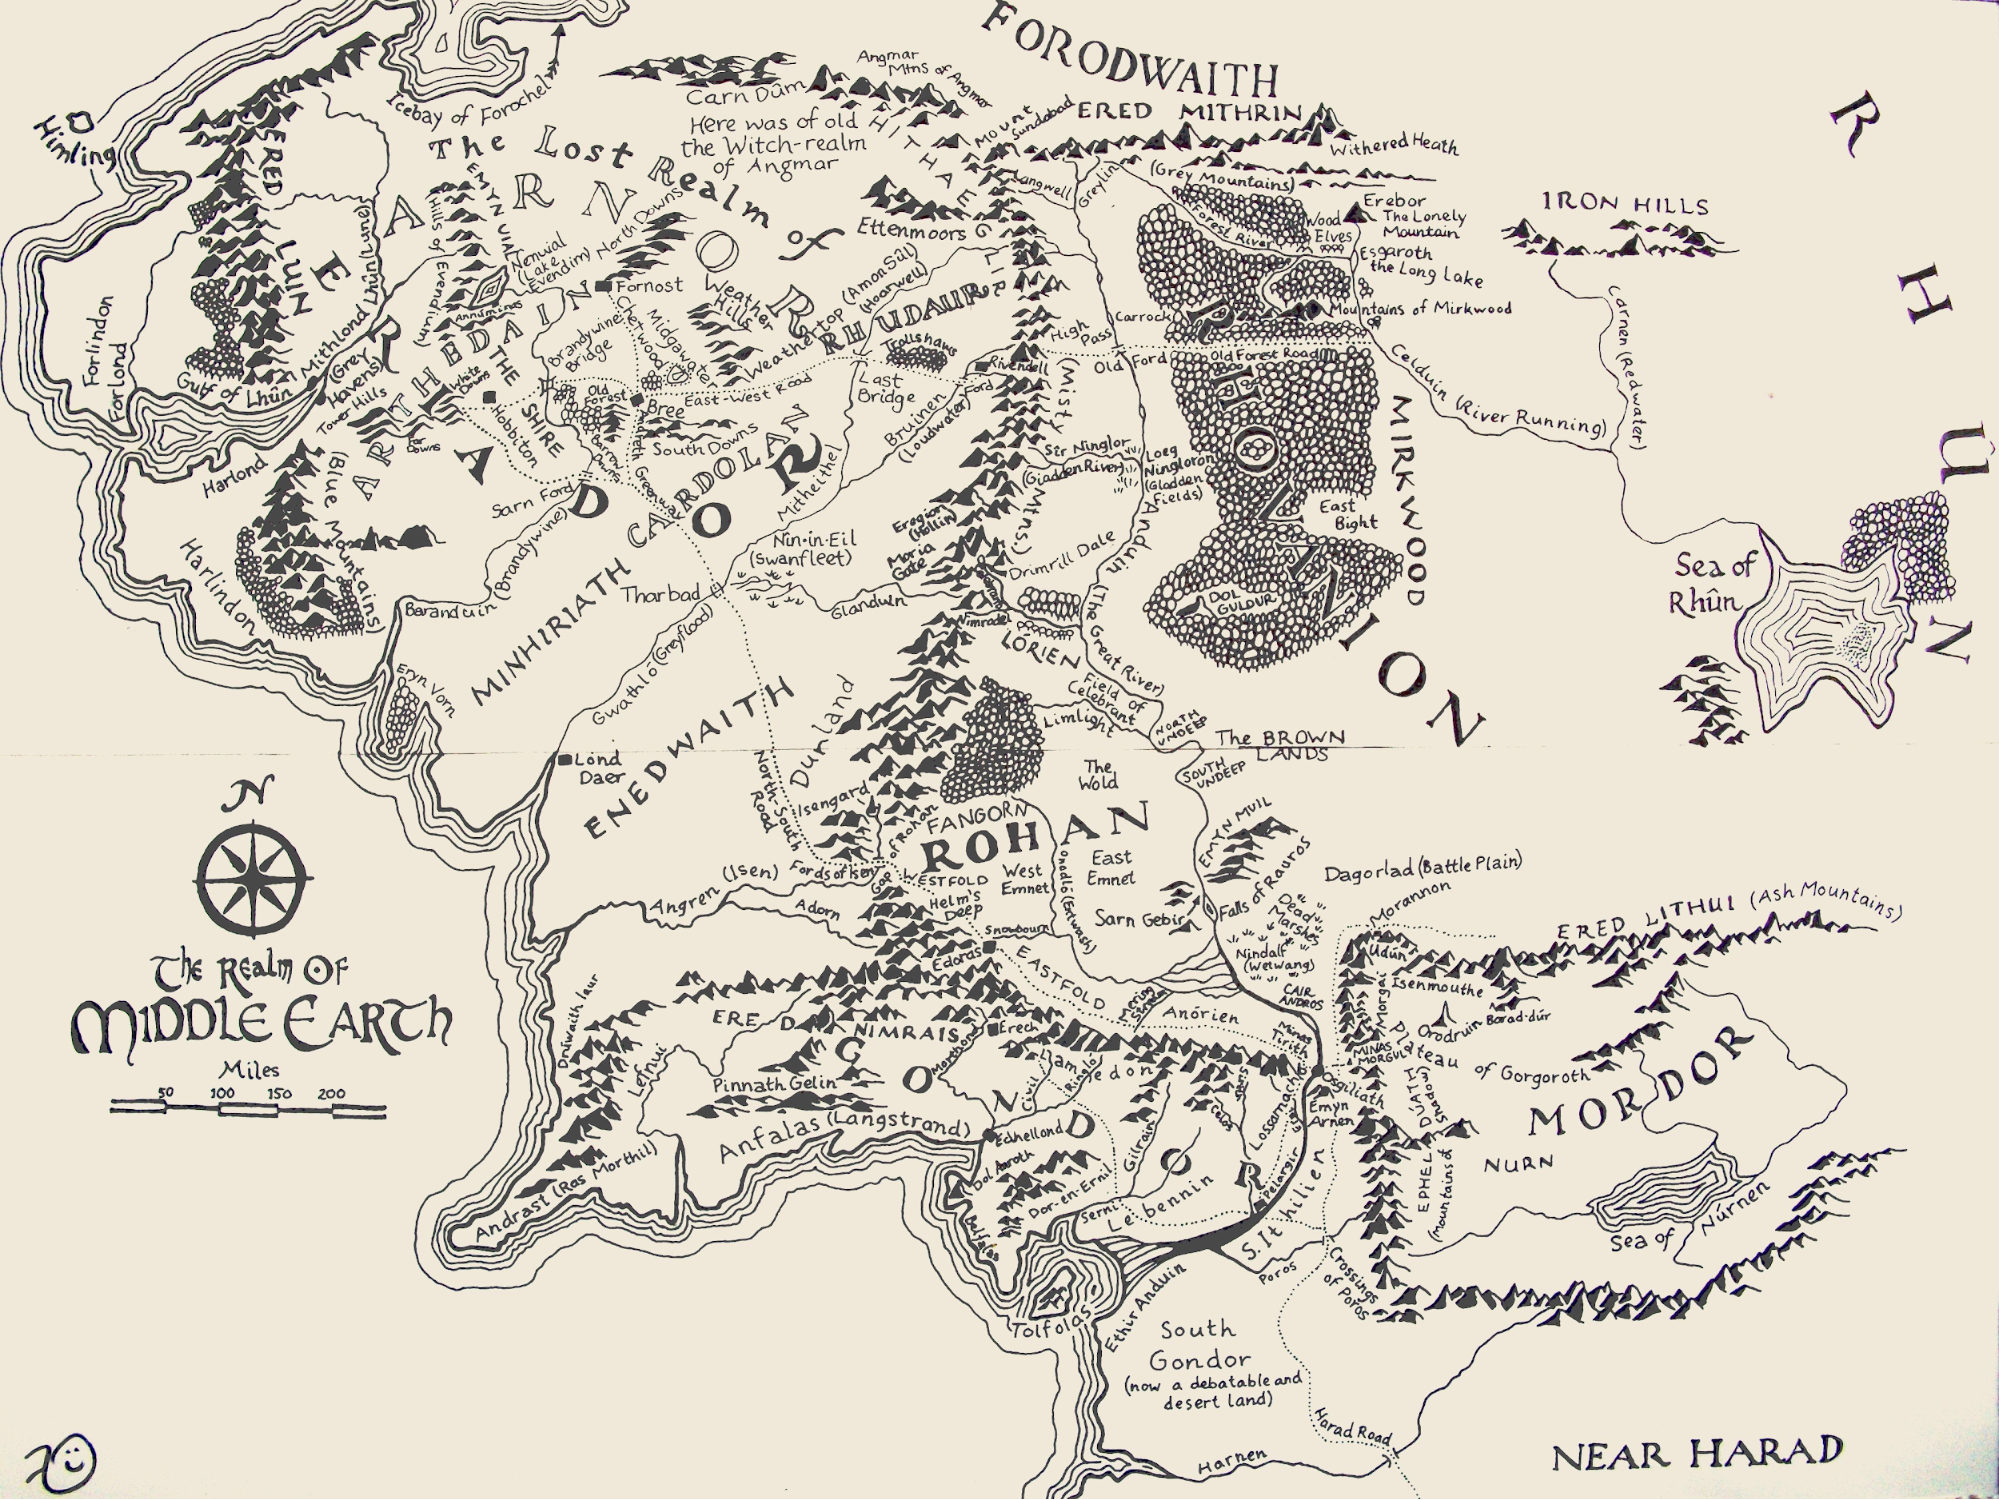
\includegraphics[scale = 0.25]{image7.png}\\
             (Note: Click the link below for a better view! \footnote{Retrived from: https://i.pinimg.com/originals/ac/9b/41/ac9b41bd405e7c5b67ab9412c958c586.jpg})
            \end{center}
            
            \newpage
            \section{Committee Background}
            
            \subsection{Creation of Middle-earth}
            
    \noindent Middle-earth is part of a larger world called Arda, which was originally created by the supreme and all-powerful deity Eru Ilúvatar. At the beginning of time Ilúvatar created fourteen god-like beings called the Valar to shape and rule the world. Ilúvatar also created angelic beings called the Maiar that were servants of the Valar, and which include such beings like Sauron and Gandalf. The Valar and Maiar are collectively referred to as the Ainur.\footnote{Arda. In The One Wiki to Rule Them All. Retrieved from https://lotr.fandom.com/wiki/Arda } \\
    
    \begin{wrapfigure} {r} {0pt}
        \centering
        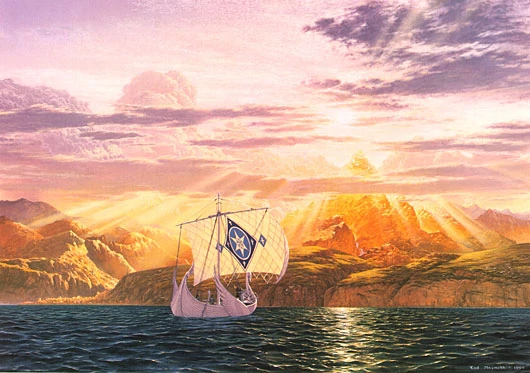
\includegraphics[scale = 0.45]{image3.png}
    \end{wrapfigure}
        
    \noindent Melkor, a powerful Valar, rebelled against Ilúvatar’s plan for the Valar to create the world and instead introduced evil into the world by stealing the Silmarils, three jewels created by the elves from the light of the Trees of Valinor. Melkor also terrorized the inhabitants of Middle-earth, spreading destruction and decay. He tortured and twisted Elves beyond recognition to form the first Orcs, who comprised a large portion of his armies for much time after. These events caused a war and ultimately the banishment of Melkor, who became known as Morgoth. The banishment of Melkor marked the end of the First Age and the beginning of the Second.\footnote{Melkor. In The One Wiki to Rule Them All. Retrieved from https://lotr.fandom.com/wiki/Melkor} \\
        
        
    \noindent The remaining fourteen Valar withdrew to the realm of Valinor, on the continent of Aman, also referred to as the Undying Lands, the Blessed Realm, or simply “The West.” In what is now known as Middle-earth, across the Great Sea from Valinor, Ilúvatar created the Children of Ilúvatar: Elves and Men (in that order). He created the elves to be beautiful, immortal, and intrinsically good, but made Men mortal and granted them free will. Other races, like Dwarves and Hobbits, were created later by the lesser deities of the Tolkien pantheon. The Orcs were not created ex nihilo, from nothing, but were actually created by Melkor prior to his banishment by torturing and twisting captured Elves into the grotesque, mortal, weak-willed, and warmongering creatures that they are today. \\
        
    \noindent Some time after the creation of the Elves and banishment of Melkor, the Valar invited the Elves to come live with them in Valinor, as they were similarly immortal and lacked the “Gift of Men.” The Gift, mortality, was bestowed onto the younger race of the Children of Ilúvatar by their creator. Mortality is what grants Men their innovative, yet corruptible, spirits.\footnote{The Gift of Men. In The One Wiki to Rule Them All. Retrieved from https://lotr.fandom.com/wiki/Gift\_of\_Men}  Some elves agreed to come to Valinor, but others remained in Middle-earth with the plan to come to Valinor at a later point. Valinor (or the “Undying Lands”) is the realm to which Frodo, Bilbo, Elrond, and Gandalf sail at the end of the War of the Ring.\footnote{Children of Iluvatar. In The One Wiki to Rule Them All. Retrieved from https://lotr.fandom.com/wiki/Children\_of\_Il\%C3\%BAvatar} By this time, most of the Elves left in Middle-earth have already left for Valinor. \\
   
\subsection{Sauron and the Rings of Power}
    
\noindent Following Morgoth’s demise, Sauron, who served him throughout his rule, inherited all of Morgoth’s evil forces and set up his own Dark Empire. To do this, he deceived the Elves into creating the Rings of Power, twenty magical rings designed to draw the leaders of the races of Middle-earth to the forces of evil and seduce them with their power. The ring Sauron created for himself, called the One Ring, was the most powerful of these rings and held influence over all the others. \\

  \begin{wrapfigure} {l} {0pt}
        \centering
        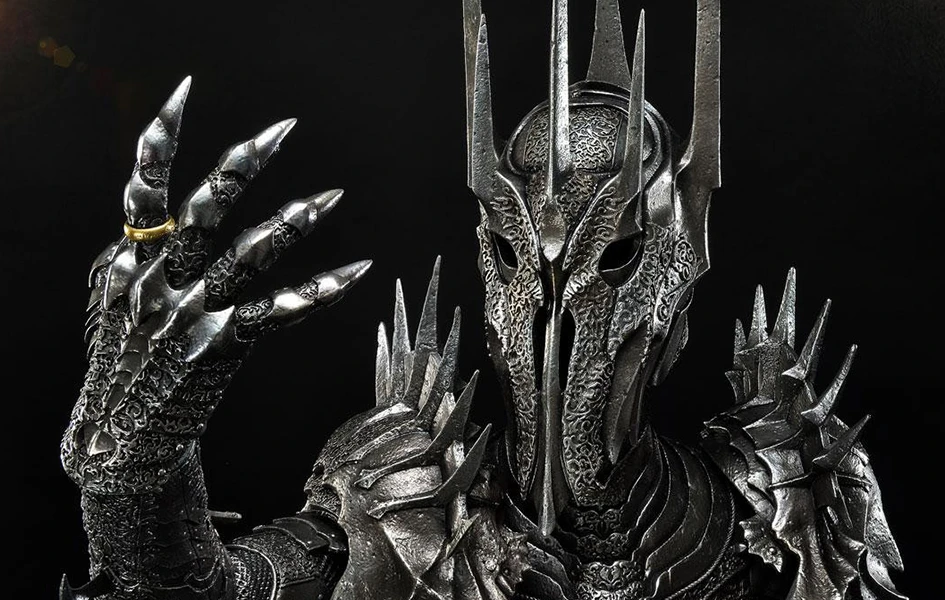
\includegraphics[scale = 0.25]{image6.png}
    \end{wrapfigure}
  
\noindent \newline However, the Ring was cut from Sauron’s finger in the War of the Last Alliance, which marked the end of the Second Age. All the events of The Hobbit and The Lord of the Rings take place during the Third Age of Arda. Sauron was substantially weakened by this initial defeat and discorporation, but he was not destroyed until Frodo dropped the One Ring into the fiery abyss of Mount Doom at the end of the War of the Ring, permanently destroying the Ring and Sauron.\footnote{Sauron. In The One Wiki to Rule Them All. Retrieved from https://lotr.fandom.com/wiki/Sauron } \\ \\

\subsection{The Wizards}

After the defeat of Melkor and his subsequent imprisonment in the Void, Manwë, leader of the Valar on Arda, learned that Melkor’s lieutenant, Sauron, was rebuilding the armies of his master and rising to power. Manwë summoned a council that decided to send five messengers to Middle-earth to protect the free peoples, reassuring them that the Valar would not forget about them.\footnote{The Wizards. In The One Wiki to Rule Them All. Retrieved from  https://lotr.fandom.com/wiki/Wizards} The Order of Wizards was sent to Middle-earth to aid the Free Peoples on the conditions that they never dominated the people of the world and that they never hoarded power like Sauron did. This was a vow that Saruman would later betray. \\

  \begin{wrapfigure} {r} {0pt}
        \centering
        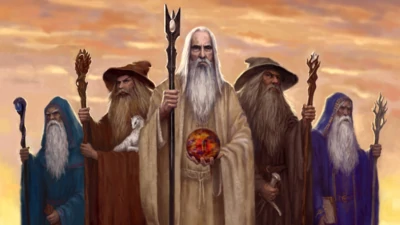
\includegraphics[scale = 0.5]{image4.png}
    \end{wrapfigure}
    
\noindent These five wizards were Maiar, immortal and primordial spirits sent to Arda to serve the Valar, incarnated into physical bodies resembling those of old men. The two Blue Wizards, Alatar and Pallando, went east before the War of the Ring, and fought alongside Dwarves, Men, and Elves in that region. Radagast the Brown lived in Mirkwood and became obsessed with living alongside and protecting plants and animals. Saruman the White and Gandalf the Grey spent their time on Middle-earth interacting with the Free Peoples. Saruman became the head of the White Council, a group of Elves and Wizards that worked to oppose Sauron. Though he was the appointed leader of the Wizards, he became jealous of Gandalf’s power and pure spirit.\\

\noindent At the end of the Third Age, after the fall of Sauron, all the Wizards except Radagast the Brown had left Middle-earth. Saruman was defeated and banished by Gandalf, and the Blue Wizards accompanied the Elves and Gandalf to Valinor. \\

\subsection{The Third Age and the War of the Last Alliance}

\noindent The Third Age of Arda began with the first defeat of Sauron at the hands of the Last Alliance of Elves and Men.\footnote{The Third Age. In The One Wiki to Rule Them All. Retrieved from https://lotr.fandom.com/wiki/Third\_Age} (Important to note, though this alliance was of “Elves and Men,” Tolkien explains that all living things were involved in the conflict).\footnote{War of the Last Alliance. In The One Wiki to Rule Them All. Retrieved from https://lotr.fandom.com/wiki/War\_of\_the\_Last\_Alliance } This war followed the downfall of the ancient human island kingdom of Numenor and the destruction of Sauron’s mortal body. At the very end of the Second Age, Elves and Men laid siege to Barad-dûr for seven years before Sauron himself emerged to fight. \\

\noindent Sauron killed High King Elendil of Gondor and Anor, the human kingdoms of the Alliance, and his son, Isildur, took up the king’s sword and cut off Sauron’s fingers and the One Ring. This dispersed the Dark Lord’s already discorporated spirit, as it was directly tied to the Ring. \\

\noindent Though Elrond implored Isildur to destroy the One Ring by casting it into the fires of Mount Doom, Isildur, being the Man that he is, fell victim to its dark influences and refused to do so. For the next 6,000 years, Sauron slowly worked to come back to power. \\

\subsection{The Events of The Hobbit}

\noindent Bilbo Baggins, the titular hobbit, is visited by his friend, the wizard Gandalf and introduced to thirteen Dwarves. He is convinced to accompany them on a quest to the Lonely Mountain, the rightful dominion of Thorin Oakenshield, the leader of the party. His decision to go on an adventure is abnormal for Hobbits, who are generally an unassuming and down-to-earth people. To reclaim the mountain, they had to defeat the dragon Smaug. \\

\noindent They proceed toward the Misty Mountains but are captured by Goblins. As they escape and flee the caverns they were brought to, Bilbo comes upon a wretched creature called Gollum living in the darkness. In the cavern, he finds a gold ring on the floor and puts it in his pocket. Unbeknownst to Bilbo, he just happened upon the One Ring, which had been lost since the beginning of the Third Age. Bilbo manages to escape Gollum after he puts the ring on his finger and becomes invisible. \\

\noindent Bilbo rejoins the dwarves, and they traverse the great forest, Mirkwood, dominion of the elven King Thranduil and home of Legolas. They stay at Laketown in Dale, where they meet Bard the Bowman, future slayer of Smaug and King of Dale. \\

  \begin{wrapfigure} {l} {0pt}
        \centering
        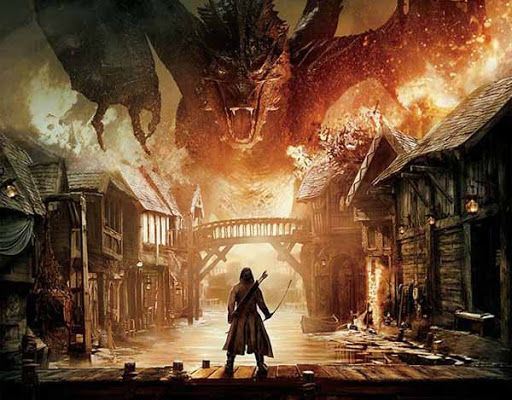
\includegraphics[scale = 0.35]{image5.png}
    \end{wrapfigure}
    
\noindent \newline Bilbo sneaks into the Lonely Mountain using the One Ring, but still manages to wake up the hibernating Smaug, narrowly avoiding death as Smaug, now enraged, leaves the mountain to destroy the surrounding area and kill all those in his path. Bard the Bowman manages to shoot down the dragon, but not before Laketown is all but burned to the ground. \\   

\noindent After the battle, Laketown makes a claim to the treasure, as do Elvish forces. The surviving Dwarves refuse to negotiate, fortifying the Lonely Mountain and summoning reinforcements from the Dwarven kingdoms. Bilbo uses the ring to turn invisible and steal the Arkenstone, the greatest treasure inside the mountain, which he takes to the besieging forces and uses to broker peace. \\

\noindent However, just as the armies (Men of Dale, Elves of Mirkwood, and Dwarves of the Iron Hills) agree to peace, they are attacked by Goblins and Wargs in retaliation for the murder of the Great Goblin during Bilbo, Gandalf, and the Dwarves’ escape from the Misty Mountains, and the Battle of the Five Armies ensues.\footnote{The Battle of Five Armies. In The One Wiki to Rule Them All. Retrieved from https://lotr.fandom.com/wiki/Battle\_of\_Five\_Armies } The newly allied forces are victorious, and the treasure is divided up amongst all parties. Although Bilbo only takes a very small portion, it makes him an incredibly wealthy hobbit, and he returns to the Shire with the Ring, unaware of its true identity. Gandalf knowingly allows Bilbo to keep the ring, as he is aware of the resistance he has to the forces of corruption as a hobbit. Not even the Grey Wizard felt that the One Ring would be safer in his own hands than in those of Bilbo Baggins. \\

\subsection{The War of the Ring}

\noindent The War of the Ring is the conflict that is told from a limited perspective in the Lord of the Rings trilogy. The southern theatre of the conflict, alongside Frodo and Sam’s Quest of Mount Doom, are the two overlapping plot arcs in the books and movies. \\

\noindent Since the dissipation of his dark spirit by Isildur in the War of the Last Alliance, Sauron had been working to regain his strength and physical form.\footnote{The War of the Ring. In The One Wiki to Rule Them All. Retrieved from https://lotr.fandom.com/wiki/War\_of\_the\_Ring } Around the time that Bilbo left the Shire and bequeathed the One Ring to Frodo, Sauron’s forces had found and captured Gollum in their search for their master’s greatest source of power. After being tortured, Gollum revealed that his precious was now in the hands of the “hobbitses” of a place called “the Shire.” \\

\noindent Sauron sent the Ringwraiths to find the Ring, forcing Gandalf and Frodo to flee to Rivendell and seek the assistance of the forces of Gondor and the Elves. There, the Fellowship of the Ring was formed, and representatives of all the Free Peoples set out on the mission to destroy the One Ring and Sauron. \\

\noindent While taking a shortcut through Mines of Moria, the Fellowship was hunted by Orcs and accidentally awakened a Balrog, a primordial fire demon that had once served Melkor in the War of Wrath before his imprisonment in the Timeless Void. In a final stand to protect the rest of the party from the beast, Gandalf was dragged from the broken Bridge of Khazad-Dum into the dark abyss beneath Moria. \\

\noindent The Balrog and Gandalf battled for days, fighting all the way up the Endless Stair and onto Durin’s Tower at the peak of the mountains.\footnote{Battle of the Peak. In The One Wiki to Rule Them All. Retrieved from  https://lotr.fandom.com/wiki/Battle\_of\_the\_Peak } The Battle of the Peak culminated in the defeat of the Balrog, but Gandalf succumbed to exhaustion and his wounds and perished. He lay on the mountainside for nineteen days until Ilúvatar himself resurrected him as Gandalf the White. He soon reunited with Aragorn, Legolas, and Gimli in Rohan. \\

\noindent The War of the Ring officially started when Saruman’s forces invaded Rohan through the Fords of Isen.\footnote{The War of the Ring. In The One Wiki to Rule Them All. Retrieved from https://lotr.fandom.com/wiki/War\_of\_the\_Ring } The battle saw the death of Theoden’s son, Theodred, the Marshal of the Westmark. This sent King Theoden of Rohan into spiraling depression. \\ 

\noindent Because of Saruman’s dark influence through Grima Wormtongue, King Theoden would not join the alliance of Men, Elves, and Dwarves until Gandalf freed the king of his curse and drove the witch out of Edoras, the seat of Rohan’s king. Together, and with the help of the Tree Ents, they defeated Saurrman’s forces at Isengard. \\

\noindent The Battle of Osgiliath was the beginning of the main push into Gondor from Mordor.\footnote{Battle of Osgilath.In The One Wiki to Rule Them All. Retrieved from https://lotr.fandom.com/wiki/Battle\_of\_Osgiliath} Though Gondor had been holding back Sauron’s forces in the east for 3000 years, this marked the beginning of the war for Gondor. The Orcs pushed Gondor’s forces all the way into the capital city of Minas Tirith and lay siege to it, starting the Siege of Gondor. \\

\noindent The Witch-king Angmar of the Nazgul actually managed to break down the gates of Minas Tirith after many failed attempts by Orcs to scale the walls. Things looked bleak for the kingdom until King Theoden himself rode into battle with 6,000 mounted Rohirrim, the cavalry forces of Rohan, to save their ally.\footnote{Battle of Pelennor Fields. In The One Wiki to Rule Them All. Retrieved from https://lotr.fandom.com/wiki/Battle\_of\_the\_Pelennor\_Field} The Battle of Pelennor Fields ensued. \\

\noindent After a day of vicious fighting, King Theoden fell, and his adopted daughter, Éowyn, successfully killed the Witch-king. In the end, the two allied kingdoms were victorious and the city was saved. From that point forward, the new King Éomer of Rohan pledged lifelong friendship between Gondor and Rohan. The vast majority of Sauron’s forces in the southern theatre were destroyed, but some were chased back to Mordor. \\

\noindent In the Northern theater, the Blue Wizards Alatar and Pallando, the Elves of Mirkwood, the Men of Dale, and the Dwarves of Erebor fought alongside one another against another large share of Sauron's total forces. They faced not just Orcs and Isengard’s Uruk-hai, but also several barbarous kingdoms of Men that were allied with the Dark Host. \\

\noindent Finally, the rest of the enemies were intent on assaulting Lothlorien, which bridged the gap between the two theatres. The Elven forces there, alongside their allies fighting Sauron in the other two theatres, were ultimately victorious because of their success in keeping the various sections of Mordor’s forces from joining one another in battle. Neither the actual fighting in Lothlorien nor the much larger battles in the northern theatre were depicted directly in the LOTR books or movies although they were essential to the ultimate victory of Sauron. \\

\noindent Finally, the real cornerstone to victory during the War of the Ring was the Quest of Mount Doom, in which Frodo Baggins and Samwise Gamgee of the Fellowship successfully destroyed the One Ring and Sauron with it. \\

\subsection{Storyline Graphic\\} 

\begin{center}
      
\includegraphics[scale = 0.3]{image1.png}\\
(Note: Click the link below for a better view! \footnote{Retrived from: https://i.pinimg.com/originals/6e/ff/a4/6effa49344a5c5614fc426688b81549f.jpg})
\end{center}

\newpage

\section{Starting Scenario: Rivendell, 3021}
\noindent As Sauron’s tower collapses at Barad-dûr, the survivors of the War of the Ring all across Middle-earth cheer, shedding tears of joy. The war is over, and the forces of darkness have been defeated. However, nothing will ever be the same in Middle-earth. Aragorn, soon to be crowned King of Gondor, pulls Gandalf the White aside while the victorious army celebrates. They know that now more than ever, the world needs guidance and order as it sets out on a new path. \\

\noindent With the War of the Ring behind them and the Ring of Power and its master destroyed, the Free People of Middle-earth must now look forward, as the Fourth Age of Arda has dawned. Gandalf, ever the steady hand that guides the realm, has set sail with the Blue Wizards, Elrond, Galadriel, Frodo, Bilbo, and the Elves of Rivendell and Lothlórien to the Undying Lands in the West. Before he left, he helped Aragorn organize a summit to plan for the future of all races. Upon his coronation at Minas Tirith, Aragorn’s first act as High King is calling together the Council of Middle-earth, which would be hosted in the neutral city of Rivendell, which has now been abandoned by the Elves. \\

\noindent The Council is made up of representatives of all races and kingdoms, even those that fought alongside Sauraun in the War. They are to decide how Middle-earth and its nations will move forward into this hopeful new age. Topics to discuss include the fate of Mordor, the Orcs and Uruk-hai, the ruins of Barad-dûr, and the Easterlings, a kingdom of Men that fought alongside Sauron in both the recent wars. They are intent on building a new and brighter future for all the citizens of the realm. \\

\newpage

\section{Questions to Consider}
\begin{enumerate}
    \item {What will be done with Mordor, Barad-dûr, and the defeated forces of Sauron?}
    \begin{itemize}
        \item {How will conquered territory and kingdoms be governed?}
        \item {Will former enemies be held to justice in some way? (Easterlings, Orcs, etc.)}
    \end{itemize}
    \item{What type of international system needs to be built to prevent future conflict and help build cohesion in Middle-earth?}
    \item{What is to come of the migration of the Elves, and what is to come of those that have stayed in Middle-earth?}
    \item{What role will the Shire play in the wider future of Middle-earth?}
\end{enumerate}

\newpage

\section{Vocabulary}

\begin{itemize}
    \item {The Rings of Power - nineteen magical rings forged by Sauron in the Second Age; three for the Elves, seven for the Dwarves, and nine for Men. Each of the rings lost their powers after the destruction of the One Ring, and the three Elven rings were taken to the Undying Lands by their wielders: Gandalf, Galadriel, and Elrond.}
    
    \item {The One Ring - created by Sauron in the fire of Mount Doom to enhance his power and control the other Rings of Power. It was destroyed by Frodo and Sam, ending the War of the Ring.}
    
    \item {Hobbits  - a mortal race whose primary dominion is the Shire; their average lifespan was about 100 years; they are about 2-3 feet tall (shorter than dwarves) with large furry feet and pointed ears. Before the War, they never involved themselves in global affairs. They are homebodies that enjoy the simple things in life. They were created by unnamed servants of Ilúvatar from Dwarven children by removing imperfections and greed from them. Their lack of desire for domination and power made them uniquely resistant to the power of the One Ring and general corruption by allies of Melkor.}
    
    \item {Elves - considered to be the fairest and wisest of the races, they are unusually beautiful and immortal, and can only die as the result of violence or despair great enough to kill their pure spirits. They were the first Children of  Ilúvatar to awaken and roam Middle-earth. }
    
    \item {Orc - bred from mutilated and corrupted elves, orcs notably served as the cruel and vicious foot soldiers of Sauron’s army. Their trauma-ridden past and Melkor’s torture made them predisposed to being bent to the will of Sauron and the Ring of Power.}
    
    \item {Uruk-hai - brutal warriors and the physically strongest soldiers in Sauron’s collective forces, Uruk-hai are rumored to be the product of cross-breeding humans and orcs. Saruman bred them in the pits of Isengard, enhancing their powers with his dark arts.}
    
    \item {Dwarves - a little taller than hobbits but far broader and heavier, Dwarves make their homes in caverns and mountains. They are master craftsmen, metallurgists, miners, and warriors.}
    
    \item {Men - the humans of Middle-earth had vastly different cultural groups spread across the land. Some kingdoms were natural enemies of Gondor and Rohan, and fought alongside Sauron’s forces in both wars.}
    
    \item {Wizards - five Maiar spirits sent to Middle-earth by Ilúvatar to aid the Free Peoples in their fight against Sauron, each is associated with a color and correspondingly ranked within the Order of Wizards. Gandalf the White is the newly ascended White Wizard.}
    
    \item {Dragons - powerful and intelligent creatures whose type was distinguished by whether they breathed fire and how they moved and who had a cunning desire for treasure}
    
    \item {Trolls - unintelligent, monstrous creatures ranging from between 10-50 feet tall, they turn to stone in sunlight}
    
    \item {Goblin - “Goblin” is the word used by Tolkein throughout The Hobbit to describe Orcs. There is a slight etymological nuance that explains why he used the word “Orc” in the trilogy, but there is no distinction between a goblin and an orc in Middle-earth.}
    
    \item {Ents - one of the oldest races of Middle-earth, Ents are strong, tree-like creatures that were taught to speak by the Elves. They protect certain forests like shepherds, and they are convinced by Merry and Pippin to attack Isengard to protect themselves and the Free Peoples. }
    
    \item {Mordor - chosen by Sauron to be his realm because of the mountains that surrounded it on three sides, Mordor is located in the southeastern part of the continent. It is a barren and desolate land, ravaged by Sauron’s armies for resources and poisoned by his dark magic. }
    
    \item {The Shire - the homeland of most of the Hobbits in Middle-earth, bound by the Brandywine River and originally divided into the four Farthings (North-, South-, East-, and Westfarthings), it has an extensive agricultural system. It survives the War of the Ring mostly untouched, but the Nazgul ravaged the land in search of the One Ring before finding it and Frodo.}
\end{itemize}

\newpage

\section{Character Descriptions}
\textbf{A note to delegates:} Some of the characters listed here were
not featured in mainstream LOTR media. Most of them were portrayed at
some point, but others were only mentioned in passing in one book or
another and fleshed out using information we could infer from other
parts of the stories. Each character is incredibly vital to the task at
hand for one reason or another, as each group of people Middle-earth
needs to have a hand in shaping the coming of the Fourth Age. Also,
\textbf{do not write to these characters in your crisis notes. They are
in the room with you.}

\begin{enumerate}
\def\labelenumi{\arabic{enumi}.}
\item
  \textbf{Éowyn} - Éowyn and her brother, Éomer, were the adopted
  children of King Théoden of Rohan, who died during the Battle of
  Pelennor Fields. Éowyn led Rohan while the king and his adopted son
  fought against Saurman and the forces of Isengard. She always had a
  longing for battle, and dressed as a man so she could fight without
  Aragorn's approval. At the Battle of the Pelennor Fields, she killed
  one of the Nazgul. After the war, she married Faramir.
\item
  \textbf{Éomer} - Éomer and his sister, Éowyn, were the adopted
  children of King Théoden of Rohan. He rode with Théoden, Aragorn, and
  Gandalf to Isengard. He went temporarily mad when he thought his
  sister, Éowyn had died, but later he joined her at the Houses of
  Healing and helped her recover from her injuries. He eventually became
  the eighteenth King of Rohan and swore everlasting friendship between
  Rohan and Gondor.
\item
  \textbf{Erkenbrand} - Erkenbrand was a warrior of Rohan during the War
  of the Ring. He returned after the death of King Théoden's son to
  command the forces of Rohan in the western regions, defending Westfold
  until summoned by Gandalf to aid forces at Helm's Deep. He is a mighty
  leader and was given the title of Marshal of the Westmark following
  the war.
\item
  \textbf{Legolas} - Legolas, son of Thranduil and Prince of Mirkwood,
  was a member of the Fellowship of the Ring. He is a master bowman, a
  great leader, and a good friend to Hobbit-, Man-, and Dwarf-kind.
  After the war, he serves as a mutual advisor to his father and
  Aragorn, acting as an informal liaison between Gondor and Mirkwood.
\item
  \textbf{Aragorn} - Aragorn II of Gondor, or King Elessar as he is now
  known, was the first high King since the short reign of Isildur. He is
  a skilled ranger and warrior. As a child, he was fostered in Rivendell
  by Elrond Half-Elven. When he was older, Elrond revealed his identity
  and gave him the Ring of Barahir and the Shards of Narsil. He fought
  alongside Legolas and Gimli, helping the people of Rohan at the Battle
  of the Hornburg. In order to defend Minas Tirith from Sauron, he
  travelled the Paths of the Dead and summoned the spirits who had to
  pay their debt after betraying Gondor in a previous age. They are now
  free. At the Battle of the Pelennor Fields, he rallied the forces of
  Gondor and Rohan to defeat Sauron's army. After the war, he was
  crowned King of Gondor and married Arwen.
\item
  \textbf{Arwen} - Daughter of Elrond, the Lord of Rivendell, and wife
  to Aragorn. Arwen, being a descendant of half-elves, chose to become
  mortal and remain in Middle-earth instead of sailing with her Elven
  brethren to the Undying Lands in order to be with Aragorn. She helped
  save Frodo by taking him to Rivendell after he was mortally wounded by
  the Nazgul.
\item
  \textbf{Gimli} - A renowned dwarf-warrior and a member of the
  Fellowship of the Ring. Originally from the mines of Moria, Gimli
  accompanied Aragorn and Legolas in their pursuit of Merry and Pippin
  when they were captured, and he fought in almost all of the major
  battles of the war. After the War of the Ring, became the first Lord
  of the Glittering Caves behind Helm's Deep. He maintains a close
  friendship with Legolas and is a very powerful and skilled warrior.
\item
  \textbf{Radagast} - The Brown Wizard, Radagast concerns himself with
  the natural world. He has a friendly relationship with the Great
  Eagles, which proved to be very useful during the War of the Ring,
  when Radagast sent them to rescue Gandalf from the tower in Isengard
  where he had been imprisoned by Saruman. Other than that, Radagast did
  not participate much in the War, instead focusing on protecting
  nature. He also possesses great healing properties.
\item
  \textbf{Meriadoc ``Merry'' Brandybuck} - Merry is a Hobbit and close
  friend to Frodo, Sam, and Pippin. He was a member of the Fellowship,
  and he and his cousin, Pippin, were captured by the Uruk-hai during
  the quest to destroy the Ring. After the pair escaped, they convinced
  the Ents to attack Isengard. Later, Merry swore fidelity to King
  Theoden of Rohan and snuck into the Battle of Pelennor Fields,
  assisting Eowyn as she killed the Witch-King of Angmar. He was later
  knighted and became a government official in the Shire, and he
  maintains good relationships with Treebeard, the Ents, Éowyn, and
  Rohan. Also, due to drinking the magical Ent-draught in Fangorn
  Forest, Merry and Pippin have grown substantially and are now the two
  tallest Hobbits in the Shire.
\item
  \textbf{Peregrin ``Pippin'' Took} - Pippin is a Hobbit and close
  friend to Sam, Frodo, and Merry. A member of the fellowship, he was
  captured by the Uruk-hai after Boromir's death, escaped with Merry,
  and joined the Ents in attacking Isengard. Following a vision in which
  Pippin encountered Sauron himself, Gandalf took him to Gondor, where
  he saved Faramir from being burned alive by his delusional father
  Denethor II. Following the War of the Ring, he was knighted and named
  a Shire government official. He, like Merry, maintains good
  relationships with Treebeard, the Ents, Éowyn, and Rohan, and is an
  unusually tall Hobbit.
\item
  \textbf{Faramir} - Brother to Boromir, second son of Denethor II, and
  Captain of the Rangers of Ithilien. He is renowned for his leadership
  and decision-making skills on the battlefield. He encountered Frodo
  and Sam on their way to destroy the Ring, but did not try to take
  advantage of the Ring's power as his brother had. Almost killed by his
  delusional father Denethor II who believed he was dead from battle
  wounds, Faramir was saved by Gandalf and Merry. He later married Eowyn
  and reigned as Steward of Gondor.
\item
  \textbf{Samwise Gamgee} - Sam is now regarded as a folk hero
  throughout Middle-earth. He helped Frodo Baggins until the very end of
  his quest to destroy the One Ring, and the world would never have been
  saved from darkness without his efforts. Sam is now the owner of Bag
  End, acts as Mayor of the Shire, and is representing the region in
  this committee.
\item
  \textbf{Shagrat} - Shagrat is the \emph{de facto} leader of the
  surviving Orcs and Uruk-hai. Though many of his kind were imprisoned,
  failing to surrender after the Siege of Barad-dûr, Shagrat represents
  those that dropped their swords on the field of battle when the Dark
  Tower fell. It is up to him to find a way for his people to live on in
  the Fourth Age alongside those they fought against. Now free of the
  influence of the One Ring, Orcs are still incredibly war-like and
  ``barbaric,'' but are not, at their core, irredeemably evil as the
  many other races of Middle-earth may believe.
\item
  \textbf{Faenor} - King of the Easterlings, a race of men that fought
  alongside Sauron's forces in Erebor against the Blue Wizards, the
  Dwarves of the Lonely Mountain, the Elves of Mirkwood, and the Men of
  Dale.
\item
  \textbf{Thorin III} - Cousin and namesake of Thorin Oakenshield of
  \emph{The Hobbit,} King Thorin III rules Erebor throughout the War of
  the Ring and into the Fourth Age. He fought alongside the Men of Dale,
  the Elves of Mirkwood, and the Blue Wizards against Sauron's forces
  heading north from Mordor and the Easterlings. Truly, these battles
  were some of the toughest during the War, as Tolkein describes their
  armies as some of the largest and most fearsome.
\item
  \textbf{Thranduil} - King of Mirkwood, Thranduil is the only Elven
  ruler to have stayed behind when Elrond, Galadriel, Frodo, Bilbo, and
  the Blue Wizards sailed to the Undying Lands. Thranduil and his Elves
  fought against the Orcs and the Easterlings alongside Dale and the
  forces of the Lonely Mountain.
\item
  \textbf{Bard II} - Bard II, King of Dale, is the great-grandson of
  Bard the Bowman, the first King of Dale after the city was destroyed
  by Smaug in the events of \emph{The Hobbit.} Bard II and the Men of
  Dale fought alongside the Blue Wizards, the Elves of Mirkwood, and the
  Dwarves of the Lonely Mountain against the forces of Sauron and the
  Easterlings.
\end{enumerate}
\end{document}
        
        
